\documentclass[aspectratio=169,10pt]{beamer}
\usetheme{metropolis}
\usepackage{appendixnumberbeamer}
\usepackage{booktabs}
\usepackage{amsmath,amssymb}
\usepackage{tikz}
\usetikzlibrary{arrows.meta,positioning,calc}
\usepackage{xcolor}
\usepackage{graphicx}
\usepackage{hyperref}
\hypersetup{colorlinks=true,urlcolor=columbia,linkcolor=columbia}

\definecolor{columbia}{RGB}{29,79,145}
\definecolor{columbialight}{RGB}{117,170,219}
\definecolor{columbiaaccent}{RGB}{210,73,42}
\definecolor{columbiagray}{RGB}{117,117,117}
\definecolor{softbg}{RGB}{245,245,250}
\definecolor{hlgreen}{RGB}{46,139,87}

\setbeamercolor{frametitle}{bg=columbia,fg=white}
\setbeamercolor{progress bar}{fg=columbiaaccent}
\setbeamercolor{alerted text}{fg=columbiaaccent}
\setbeamercolor{block title}{bg=columbia,fg=white}
\setbeamercolor{block body}{bg=softbg}
\setbeamerfont{title}{size=\Large,series=\bfseries}
\setbeamerfont{subtitle}{size=\normalsize}
\graphicspath{{./figures/}}

\title{Lecture 26: Proteins, Molecules \& Structural Biology}
\subtitle{BINF 4002 --- Machine Learning for Health}
\author{Matthew McDermott}
\institute{Dept.\ of Biomedical Informatics, Columbia University}
\date{Spring 2026}

\begin{document}

\begin{frame}[noframenumbering]
\maketitle
\end{frame}

% ============================================================
\begin{frame}{Where We Are}
\textbf{Three lectures on biological \& molecular data:}
\begin{itemize}
    \item[\textcolor{columbiagray}{$\bullet$}] L25: DNA, Genetics \& Gene Regulation --- genome-level biology + classical statistics
    \item[\textcolor{columbiaaccent}{$\to$}] \alert{L26: Proteins, Molecules \& Structural Biology} $\gets$ \textbf{today}
    \item[\textcolor{columbiagray}{$\circ$}] L27: Modern Biological AI --- deep learning across all levels
\end{itemize}

\vspace{0.3em}
\textbf{Same pattern as L25:} biology interleaved with methods.

\vspace{0.2em}
\textbf{Today:} Two molecular levels, each with their classical toolkit.
\begin{enumerate}
    \item \textbf{Proteins:} sequences $\to$ alignment $\to$ conservation $\to$ variant prediction $\to$ structure
    \item \textbf{Small molecules:} representations $\to$ fingerprints $\to$ QSAR $\to$ docking
\end{enumerate}

\vspace{0.2em}
{\small These are the methods your DL models in L27 need to beat---and they're surprisingly hard to beat.}
\end{frame}

% ============================================================
\section{Protein Biology}
% ============================================================

\begin{frame}{From DNA to Protein}
\begin{center}
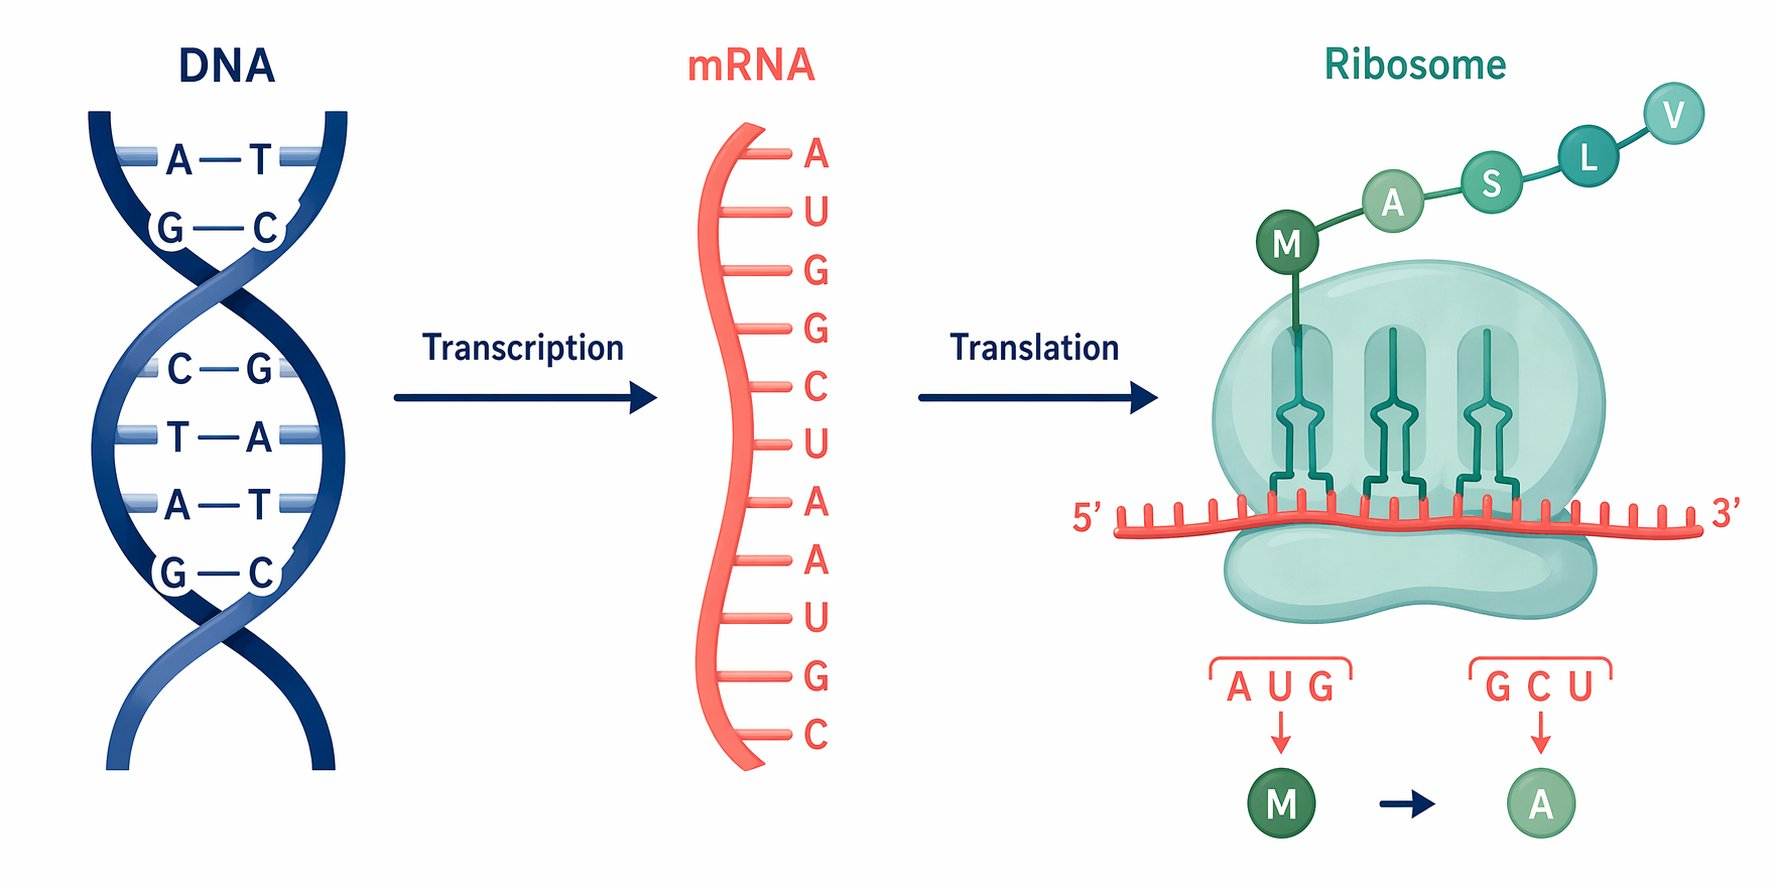
\includegraphics[width=\textwidth,height=0.50\textheight,keepaspectratio]{dna_to_protein.png}
\end{center}

\vspace{-0.2em}
{\small DNA is transcribed to mRNA, then translated into protein by the ribosome. Each \textbf{codon} (3 nucleotides) specifies one amino acid. 64 codons $\to$ 20 amino acids + stop signals.}

\vspace{0.2em}
{\small \textbf{L25 covered the DNA side.} Today: what happens after translation---the proteins and small molecules that do the work.}
\end{frame}

% ============================================================
\begin{frame}{The Genetic Code}
\begin{center}
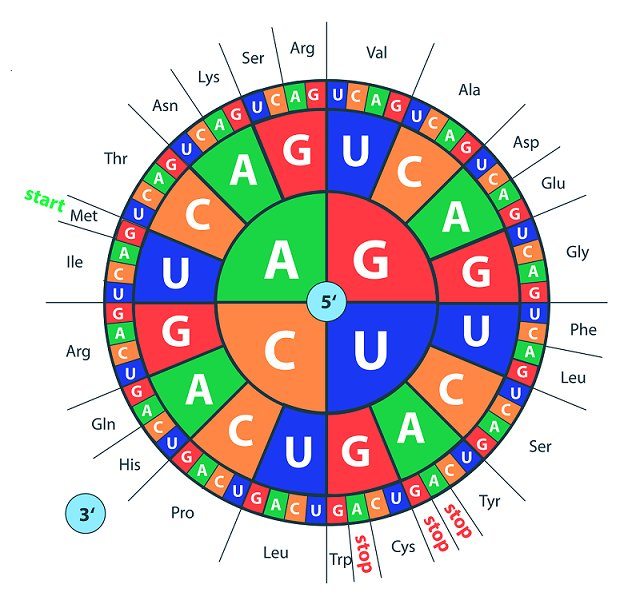
\includegraphics[width=0.65\textwidth,height=0.80\textheight,keepaspectratio]{codon_wheel.png}
\end{center}
\end{frame}

% ============================================================
\begin{frame}{What Is a Protein?}
\textbf{A sequence of amino acids from a 20-letter alphabet.}

\vspace{0.2em}
\begin{center}
\texttt{M\textcolor{columbiaaccent}{V}HLTP\textcolor{columbia}{E}EKSAV\textcolor{columbiaaccent}{T}ALWGK\textcolor{columbia}{V}NV\textcolor{columbiaaccent}{D}EVGG\textcolor{columbia}{E}ALGR\textcolor{columbiaaccent}{L}LVV\textcolor{columbia}{Y}PWTQ\textcolor{columbiaaccent}{R}...}
\end{center}
{\scriptsize Human hemoglobin $\beta$-chain (HBB), 147 residues.}

\vspace{0.2em}
\textbf{The NLP analogy:}
\begin{center}
{\small
\begin{tabular}{lll}
\toprule
\textbf{NLP concept} & \textbf{Protein analogue} & \textbf{Why it matters} \\
\midrule
Token & Amino acid (20 types) & Small vocabulary, no spaces \\
Word / n-gram & Motif (e.g., binding site) & Functional units \\
Phrase & Domain (${\sim}50$--$300$ residues) & Modular building blocks \\
Grammar & 3D fold constraints & Physics, not convention \\
Corpus & UniProt ($>$200M seqs) & Massive unlabeled data \\
\bottomrule
\end{tabular}}
\end{center}
\end{frame}

% ============================================================
\begin{frame}{The Four Levels of Protein Structure}
\begin{center}
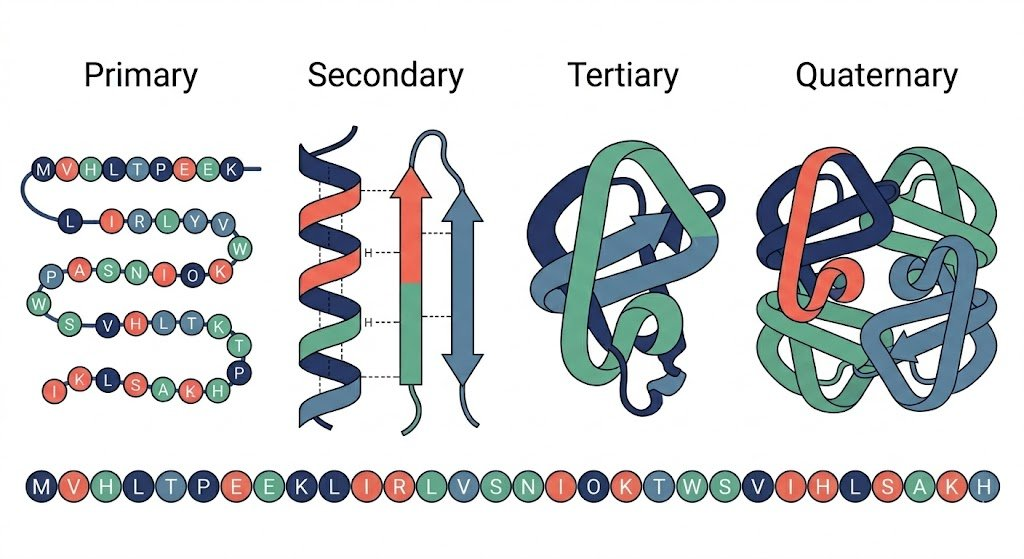
\includegraphics[width=\textwidth,height=0.36\textheight,keepaspectratio]{protein_structure_levels.png}
\end{center}

\vspace{-0.2em}
\alert{Sequence strongly constrains structure, which strongly constrains function.}

{\footnotesize (Environment, chaperones, PTMs, and binding partners also matter---but sequence is the starting point.)}

\pause
\vspace{0.1em}
{\footnotesize
\begin{itemize}\itemsep0em
    \item Single amino acid change can dramatically alter behavior (sickle cell: E6V promotes HbS polymerization)
    \item Protein misfolding $\to$ disease (e.g., CFTR F508del in cystic fibrosis)
    \item Drugs bind specific 3D shapes $\to$ know the structure, design the drug
\end{itemize}
}
\end{frame}

% ============================================================
\begin{frame}{Experimental Structure Determination}
\begin{center}
{\normalsize
\renewcommand{\arraystretch}{1.4}
\begin{tabular}{lp{8cm}}
\toprule
\textbf{Method} & \textbf{Characteristics} \\
\midrule
X-ray crystallography & Most PDB entries; requires crystals; often very high resolution \\
Cryo-EM & Growing fast; especially powerful for large complexes; no crystals needed \\
NMR & Solution-state ensembles; smaller systems; uniquely captures dynamics \\
\bottomrule
\end{tabular}
}
\end{center}

\vspace{0.5em}
Each has \textbf{biases}: what crystallizes $\neq$ what's most important biologically. Resolution varies by method and target. Cryo-EM has surged since ${\sim}$2015 (see Notebook Fig.~1).
\end{frame}

% ============================================================
\begin{frame}{The Protein Data Gap}
\textbf{The defining data challenge in protein biology:}

\vspace{0.3em}
\begin{itemize}[<+->]\itemsep0.4em
    \item \textbf{Sequences:} $>$200 million in UniProt --- massive, mostly unlabeled
    \item \textbf{Experimental structures:} ${\sim}$250 thousand in PDB --- tiny by comparison (${\sim}0.1\%$)
    \item \textbf{Function labels:} ClinVar (clinical variants), DMS/MaveDB (experimental assays) --- sparse but growing
    \item \textbf{Predicted structures:} ${\sim}$200 million from AlphaFold DB --- but predictions $\neq$ ground truth
\end{itemize}

\vspace{0.3em}
{\small This ratio screams ``self-supervised pre-training'' (L27). Before 2020, the sequence--structure gap was partially filled by classical methods. Understanding these is essential to understanding why AlphaFold~2 was a breakthrough.}
\end{frame}

% ============================================================
\begin{frame}{Evolutionary Relationships}
\begin{columns}[T]
\column{0.55\textwidth}
\begin{center}
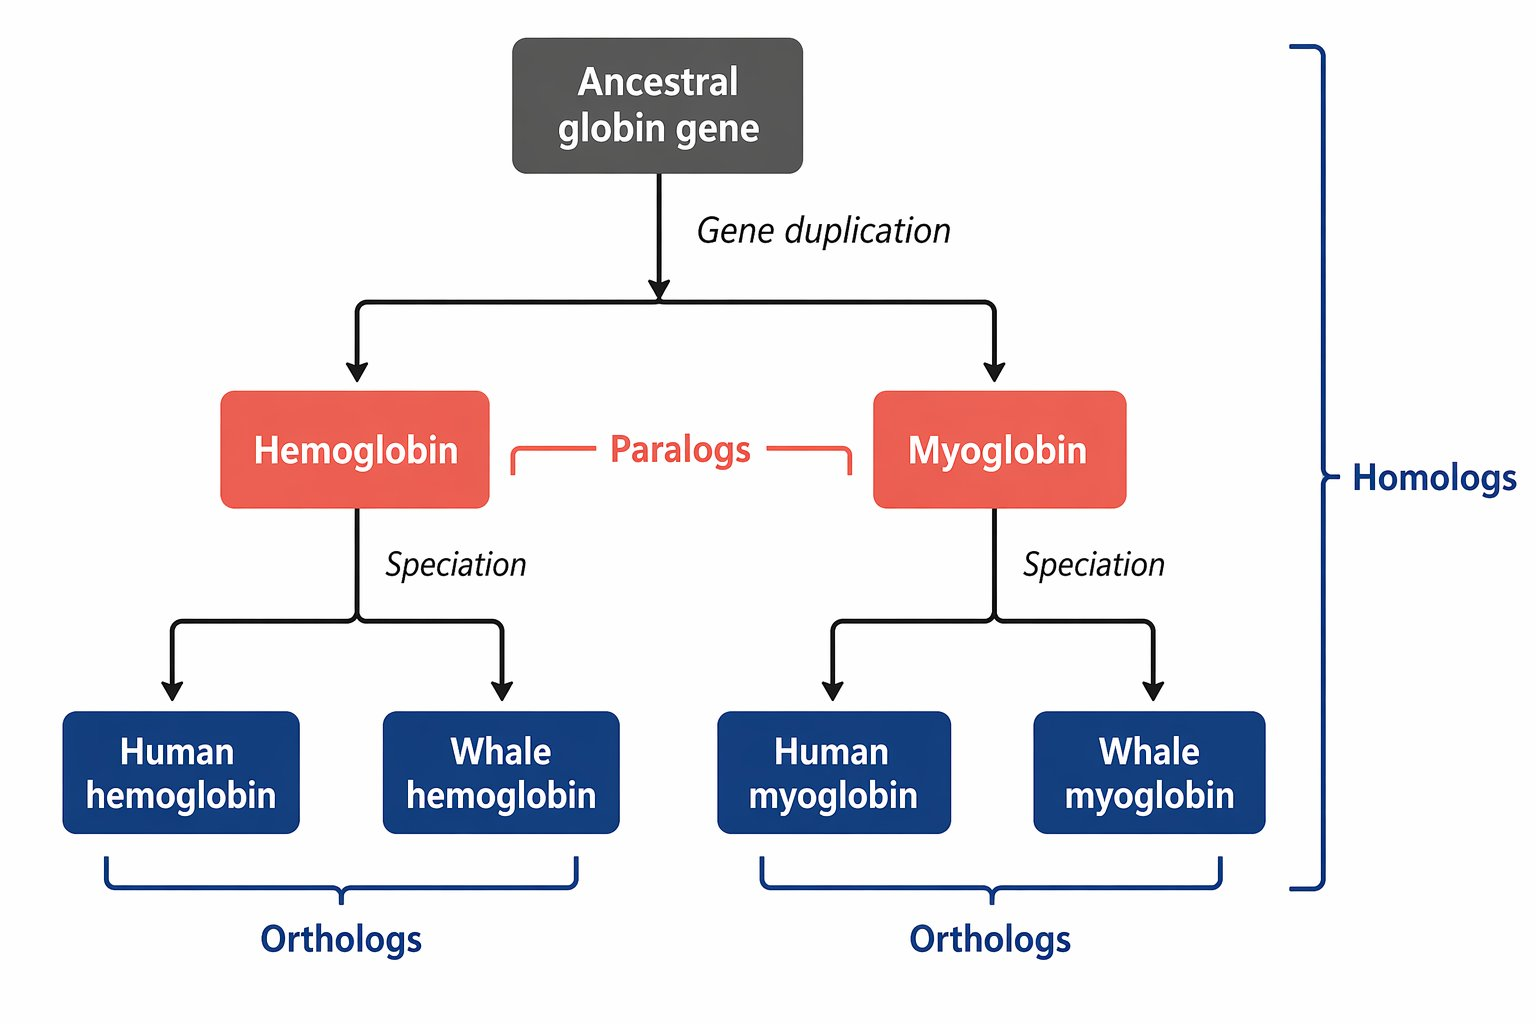
\includegraphics[width=\textwidth,height=0.70\textheight,keepaspectratio]{evolutionary_tree.png}
\end{center}

\column{0.42\textwidth}
\vspace{1em}
{\small
\textbf{Orthologs} (speciation): usually conserve function.

\vspace{0.3em}
\textbf{Paralogs} (gene duplication): may diverge in function.

\vspace{0.3em}
All are \textbf{homologs}. Even distant homologs can share the same 3D fold---structure is more conserved than sequence.

\vspace{0.5em}
\textbf{Conserved positions} = functional constraint.

\textbf{Variable positions} = often more tolerated, but can matter in specific contexts.
}
\end{columns}
\end{frame}

% ============================================================
\section{Classical Protein Analysis}
% ============================================================

\begin{frame}{Sequence Alignment: The Fundamental Operation}
\textbf{Pairwise alignment:} match, mismatch, gap.
\vspace{0.1em}
\begin{center}
\texttt{%
\textcolor{hlgreen}{M}\textcolor{hlgreen}{V}\textcolor{hlgreen}{H}\textcolor{hlgreen}{L}\textcolor{hlgreen}{T}\textcolor{hlgreen}{P}\textcolor{columbiagray}{-}\textcolor{hlgreen}{E}\textcolor{hlgreen}{E}\textcolor{hlgreen}{K}...} \\[0.1em]
\texttt{%
\textcolor{hlgreen}{M}\textcolor{columbiaaccent}{L}\textcolor{hlgreen}{H}\textcolor{hlgreen}{L}\textcolor{columbiaaccent}{S}\textcolor{hlgreen}{P}\textcolor{columbiagray}{G}\textcolor{hlgreen}{E}\textcolor{hlgreen}{E}\textcolor{hlgreen}{K}...}
\end{center}

\vspace{0.1em}
{\small \textbf{BLOSUM62:} observed substitution frequencies. Intuition: ``V $\to$ L is cheap, V $\to$ P is expensive.''}

\vspace{0.1em}
{\small \textbf{Two modes:}
\begin{itemize}\itemsep0em
    \item \textbf{Global} (Needleman-Wunsch): align entire sequences end-to-end
    \item \textbf{Local} (Smith-Waterman): find best-matching subsequence---used by BLAST, MMseqs2
\end{itemize}
}

\pause
\vspace{0.1em}
{\small \textbf{Beyond pairwise:} Profile HMMs (HHsearch, HMMER) model position-specific residue distributions---more sensitive for remote homologs; used in AlphaFold~2's MSA pipeline.}
\end{frame}

% ============================================================
\begin{frame}{Multiple Sequence Alignment (MSA)}
\textbf{Align $N$ homologous sequences.} The foundation of classical protein analysis.

\vspace{0.2em}
\begin{center}
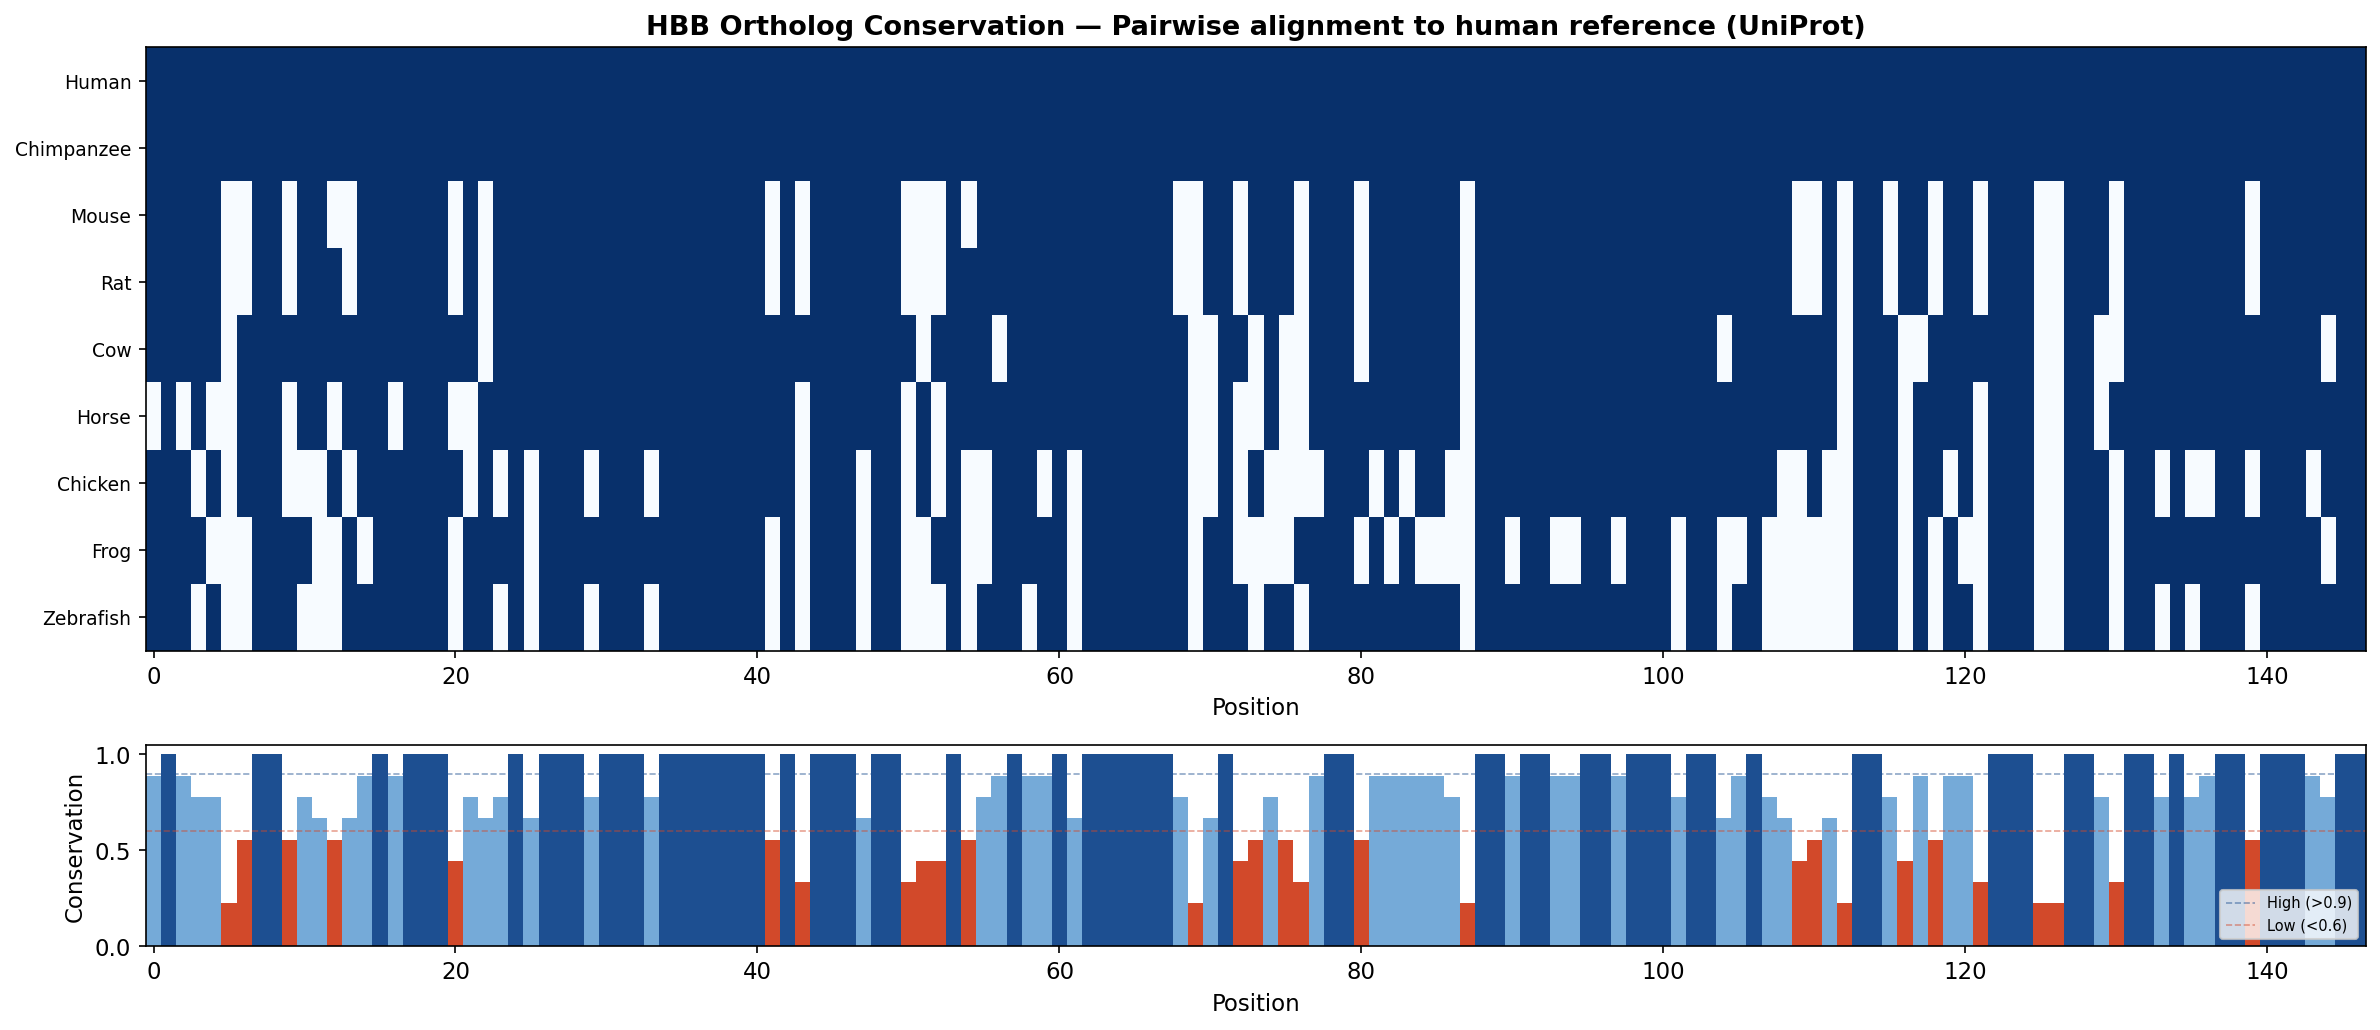
\includegraphics[width=0.95\textwidth,height=0.55\textheight,keepaspectratio]{fig2_msa_conservation.png}
\end{center}
\vspace{-0.5em}
{\scriptsize [Notebook Fig.~2] Positional identity across 9 vertebrate HBB orthologs (UniProt). Dark = identical. Light = divergent. Everything downstream---conservation, coevolution, variant prediction, homology modeling---flows from the MSA. (This is a simplified conservation view; full MSA tools like Clustal Omega jointly optimize the alignment.)}
\end{frame}

% ============================================================
\begin{frame}{PSSMs and Coevolution}
\begin{columns}[T]
\column{0.48\textwidth}
\textbf{Position-Specific Scoring Matrices:}
{\small
\begin{itemize}\itemsep0em
    \item At each MSA position, compute probability of each amino acid
    \item Encodes which substitutions are tolerated \emph{at that position}
    \item Used for: variant scoring, PSI-BLAST
    \item \textbf{Limitation:} positions scored independently---ignores context
\end{itemize}
}

\column{0.48\textwidth}
\textbf{Coevolution \& Contact Prediction:}
{\small
\begin{itemize}\itemsep0em
    \item Positions that mutate \emph{together} $\to$ often in physical contact
    \item Direct Coupling Analysis (DCA)
    \item \alert{AlphaFold~2 explicitly uses} MSA coevolution; protein LMs may recover related signals implicitly
\end{itemize}
}
\end{columns}

\pause
\vspace{0.2em}
\begin{block}{Intuition}
{\small If positions 12 and 85 always change together across species, they are probably in 3D contact. The MSA contains implicit structural information.}
\end{block}
\end{frame}

% ============================================================
\begin{frame}{The Variant Effect Problem}
\textbf{A mutation changes the DNA sequence. What happens to the protein?}

\vspace{0.3em}
\begin{center}
{\small
\renewcommand{\arraystretch}{1.3}
\begin{tabular}{lll}
\toprule
\textbf{Variant type} & \textbf{What happens} & \textbf{Likely impact} \\
\midrule
\textbf{Synonymous} & Different codon, same amino acid & Usually neutral (but not always) \\
\textbf{Missense} & Different amino acid at one position & Ranges from benign to lethal \\
\textbf{Nonsense} & Premature stop codon & Usually loss of function \\
\textbf{Frameshift} & Insertion/deletion shifts reading frame & Usually loss of function \\
\bottomrule
\end{tabular}
}
\end{center}

\pause
\vspace{0.2em}
{\small \textbf{The key question for clinical genetics:} given a missense variant, is it benign or pathogenic? This is the \emph{variant effect prediction} problem---and it is where conservation from the MSA becomes directly useful.}
\end{frame}

% ============================================================
\begin{frame}{Classical Variant Effect Prediction}
\textbf{Pre-DL methods --- many still used in clinical genetics:}

\vspace{0.3em}
\begin{center}
{\small
\renewcommand{\arraystretch}{1.3}
\begin{tabular}{lp{5.5cm}p{3.5cm}}
\toprule
\textbf{Method} & \textbf{Approach} & \textbf{Scope} \\
\midrule
SIFT & MSA conservation $\to$ continuous score & Missense variants \\
PolyPhen-2 & Sequence + structural features & Missense variants \\
CADD & Integrates $>60$ annotations & All variant types \\
REVEL & Ensemble of missense-specific scores & Missense variants \\
\bottomrule
\end{tabular}
}
\end{center}

\pause
\vspace{0.2em}
{\small A shared signal is \textbf{evolutionary conservation}, though these methods differ substantially in what additional features they incorporate. In current practice, integrative scores (REVEL, CADD) and DL methods (AlphaMissense) are increasingly preferred.}
\end{frame}

% ============================================================
\begin{frame}{Variant Effect Prediction: Conservation in Action}
\begin{center}
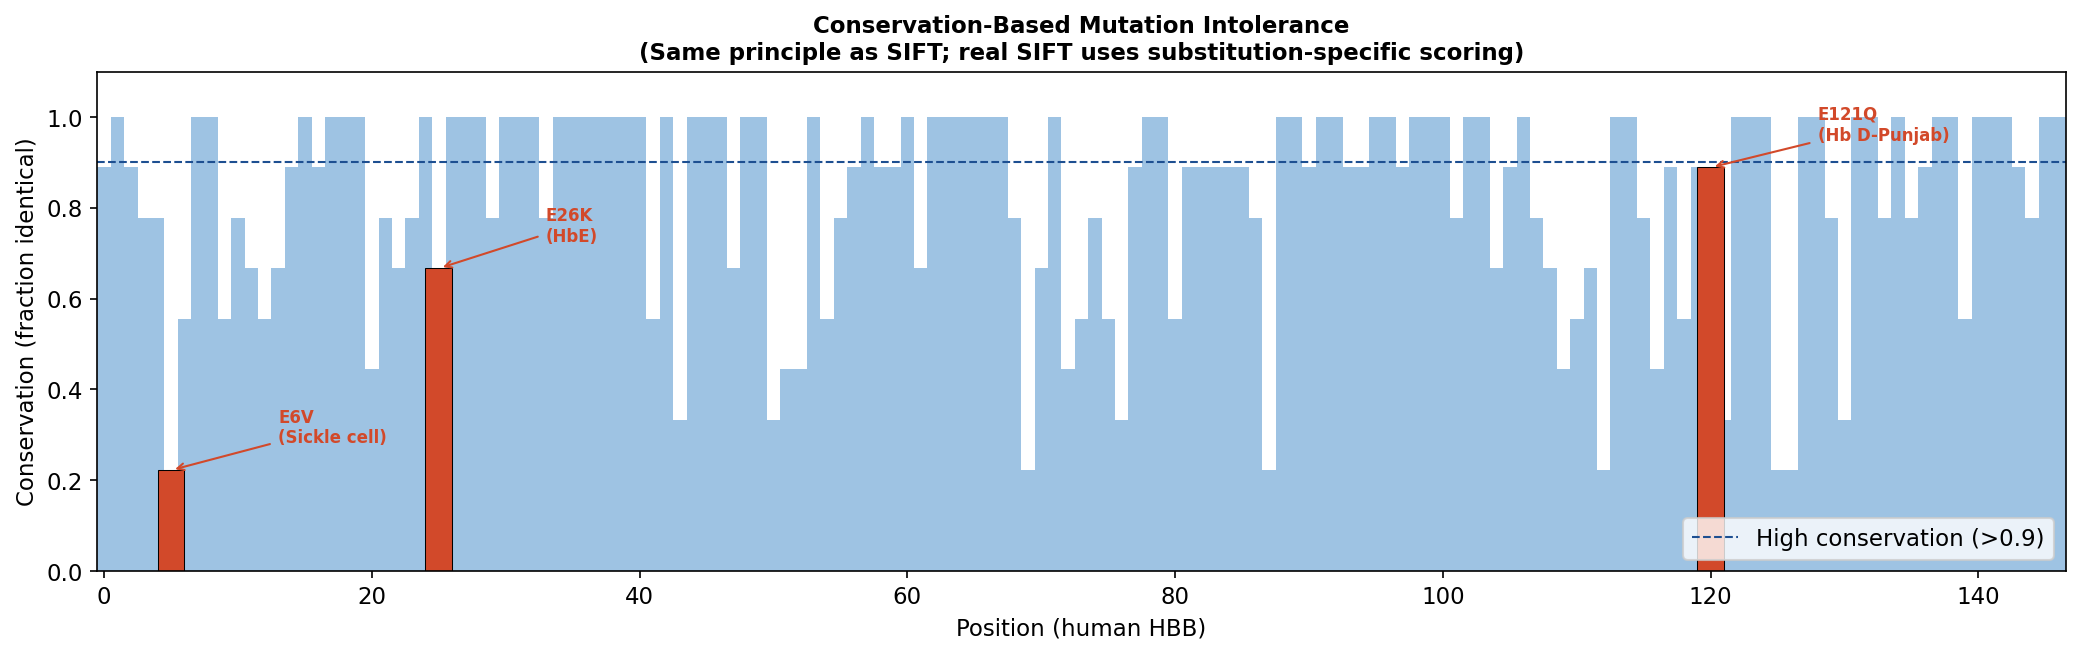
\includegraphics[width=0.95\textwidth,height=0.70\textheight,keepaspectratio]{fig3_conservation_score.png}
\end{center}
\vspace{-0.5em}
{\scriptsize [Notebook Fig.~3] Conservation across HBB orthologs. Highly conserved positions (dark blue) are intolerant of substitution---mutations there are more likely damaging. This is the principle underlying SIFT; real SIFT uses substitution-specific scoring from the full MSA.}
\end{frame}

% ============================================================
\begin{frame}{Homology Modeling: Predicting Structure Before AlphaFold}
\textbf{Task:} Given a protein sequence with unknown structure, predict its 3D fold.

\vspace{0.2em}
\textbf{Classical approach:} If a homolog with roughly $>$30\% sequence identity has a solved structure, use it as a template.

\vspace{0.2em}
\begin{center}
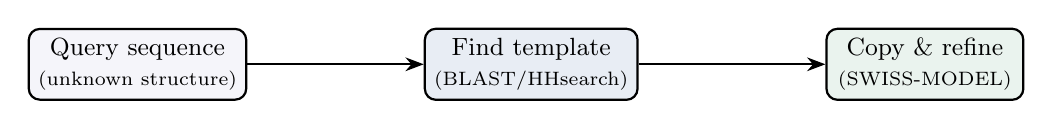
\begin{tikzpicture}[
    box/.style={draw,thick,rounded corners,minimum width=2.5cm,minimum height=0.85cm,align=center,font=\small},
    >=Stealth
]
\node[box,fill=softbg] (query) at (0,0) {Query sequence\\{\scriptsize (unknown structure)}};
\node[box,fill=columbia!10] (align) at (5,0) {Find template\\{\scriptsize (BLAST/HHsearch)}};
\node[box,fill=hlgreen!10] (model) at (10,0) {Copy \& refine\\{\scriptsize (SWISS-MODEL)}};
\draw[->,thick] (query) -- (align);
\draw[->,thick] (align) -- (model);
\end{tikzpicture}
\end{center}

\vspace{0.2em}
\textbf{Limitation:} Fails for novel folds (no template). Before AlphaFold~2 (2020), ${\sim}$30\% of protein families had no structural template.

\vspace{0.2em}
\begin{block}{The Protein Analysis Toolkit (Summary)}
MSA $\to$ conservation / coevolution $\to$ variant prediction / homology modeling.\\
\emph{Everything flows from the MSA.}
\end{block}
\end{frame}

% ============================================================
\begin{frame}[standout]
    \large If proteins are the machinery of the cell,\\[0.5em]
    how do we design molecules to interact with them?\\[1em]
    \normalsize Small molecules are \emph{one} answer---\\
    biologics, gene therapies, and antibodies are others.
\end{frame}

% ============================================================
\section{Small Molecules}
% ============================================================

\begin{frame}{Molecular Representations: Three Different Ways}
\begin{columns}[T]
\column{0.40\textwidth}
\begin{center}
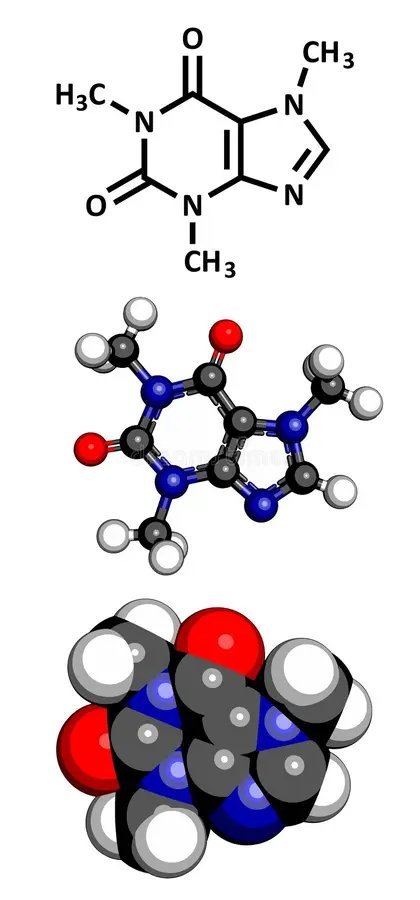
\includegraphics[width=\textwidth,height=0.78\textheight,keepaspectratio]{molecule_representations.png}
\end{center}

\column{0.55\textwidth}
\vspace{0.5em}
{\small \textbf{Caffeine} shown three ways:}

\vspace{0.3em}
\textbf{2D Skeletal} (top)\\
{\small The chemist's standard notation.}

\vspace{0.3em}
\textbf{Ball-and-stick} (middle)\\
{\small Atoms and bonds in 3D. Shows geometry.}

\vspace{0.3em}
\textbf{Space-filling} (bottom)\\
{\small Van der Waals radii. Shows molecular shape.}

\vspace{0.5em}
\textbf{SMILES string:}\\
{\small \texttt{Cn1c(=O)c2c(ncn2C)n(C)c1=O}}

\vspace{0.3em}
{\footnotesize Representation choice $\to$ model family:\\SMILES $\to$ sequence models\\Graph $\to$ GNNs\\3D coordinates $\to$ equivariant networks}
\end{columns}
\end{frame}

% ============================================================
\begin{frame}{SMILES: Molecules as Strings}
\textbf{SMILES} (Simplified Molecular-Input Line-Entry System):
\begin{itemize}
    \item Atoms $\to$ element symbols: \texttt{C}, \texttt{N}, \texttt{O}, \texttt{S}
    \item Branches $\to$ parentheses: \texttt{C(=O)O}
    \item Rings $\to$ digit pairs: \texttt{c1ccccc1} (benzene)
    \item Chirality $\to$ \texttt{@}, \texttt{@@} (but often omitted)
\end{itemize}

\vspace{0.2em}
{\small Aspirin: \texttt{CC(=O)Oc1ccccc1C(=O)O}}

\vspace{0.3em}
\begin{block}{Representation $\to$ Model Family}
SMILES (1D text) $\to$ sequence models. Graph (2D: atoms = nodes, bonds = edges) $\to$ GNNs. 3D coordinates $\to$ equivariant networks (L27).
\end{block}

\vspace{0.1em}
{\small \textbf{Limitations:} Not unique (multiple valid SMILES per molecule). Chirality notation exists but is often omitted. No explicit 3D information.}
\end{frame}

% ============================================================
\begin{frame}{Chirality: Why 3D Shape Matters}
\begin{center}
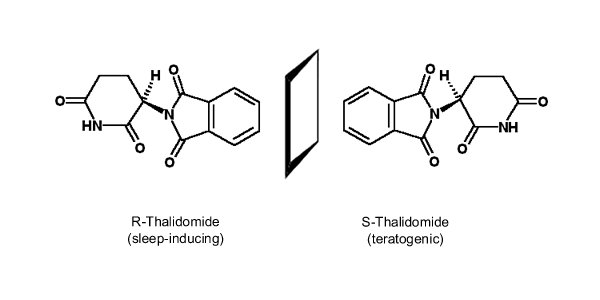
\includegraphics[width=0.80\textwidth,height=0.45\textheight,keepaspectratio]{chirality.png}
\end{center}

\vspace{-0.2em}
{\small \textbf{Enantiomers:} non-superimposable mirror images at a chiral center. Identical 2D structure, different 3D handedness $\to$ different biological effects.}

\pause
\vspace{0.2em}
{\small \textbf{Thalidomide:} R-enantiomer is sleep-inducing; S-enantiomer is teratogenic. But they interconvert in vivo---you cannot simply administer ``the safe one.'' This is why 2D representations (SMILES, fingerprints) lose critical information for drug design.}
\end{frame}

% ============================================================
\begin{frame}{Molecular Fingerprints}
\textbf{Morgan/ECFP fingerprints:} hash local substructures into binary vectors.

\vspace{0.2em}
{\small
\begin{enumerate}\itemsep0em
    \item Walk outward from each atom (radius 2--3 bonds)
    \item Hash each substructure $\to$ set bit in vector (e.g., 2048 bits)
    \item \textbf{Tanimoto similarity:} $\frac{|A \cap B|}{|A \cup B|}$ for comparing molecules
\end{enumerate}
}

\pause
\vspace{0.2em}
{\small \alert{Activity cliffs:} molecule pairs with high Tanimoto similarity but dramatically different potency. Fingerprints miss subtle structural changes that flip biological activity.}

\pause
\vspace{0.2em}
{\small \alert{Still competitive!} FP + RF/XGBoost often beats GNNs on small datasets.}
\end{frame}

% ============================================================
\begin{frame}{Fingerprint Similarity in Practice}
\begin{center}
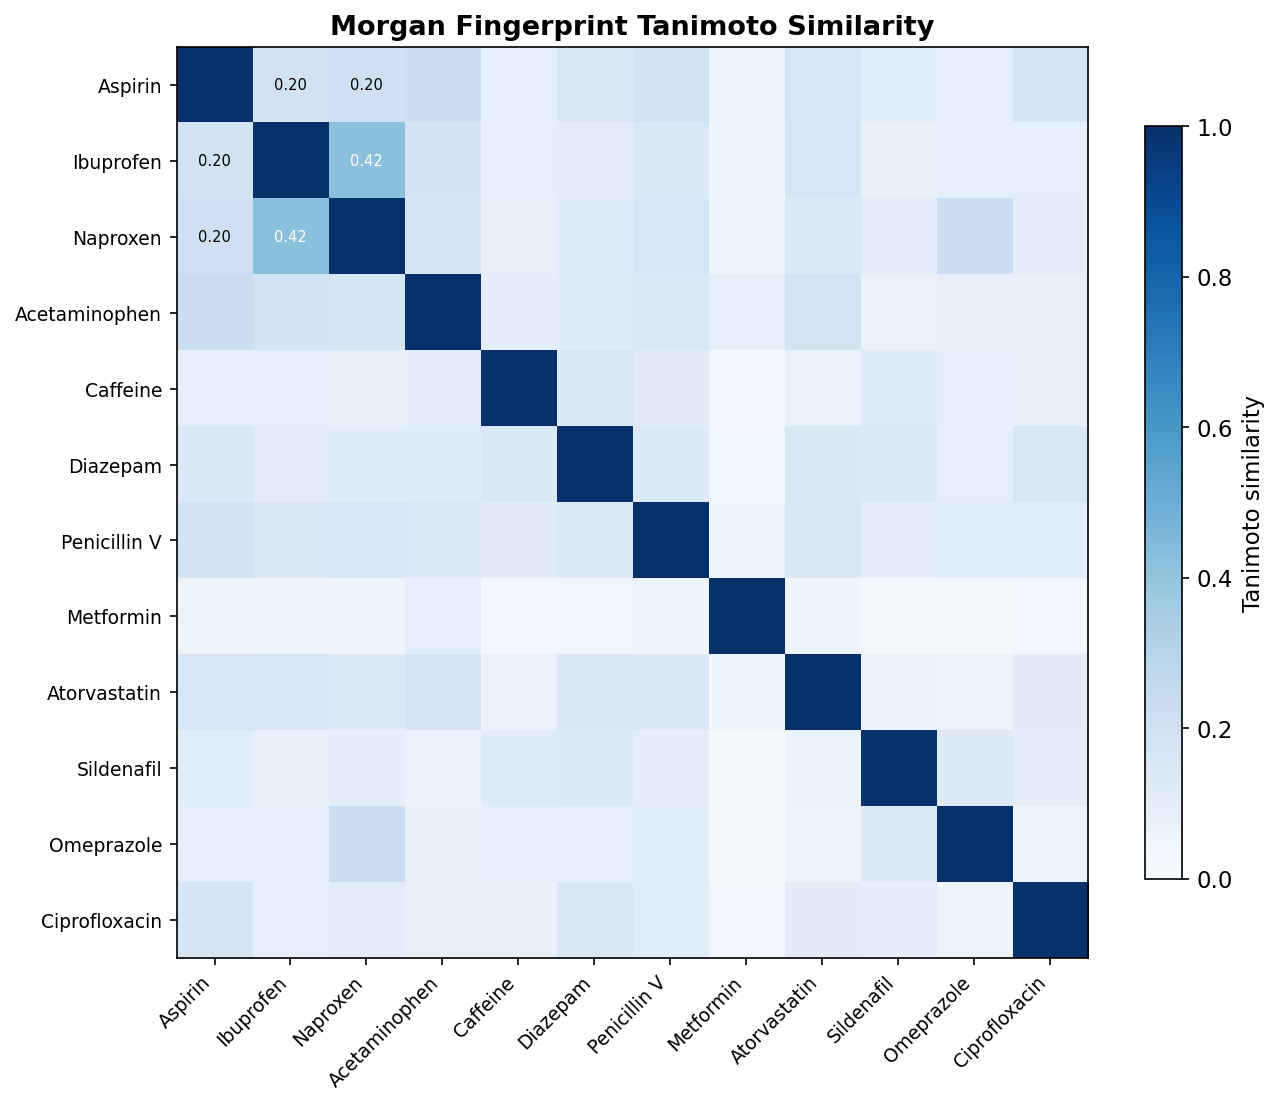
\includegraphics[width=0.90\textwidth,height=0.68\textheight,keepaspectratio]{fig4_fingerprint_similarity.png}
\end{center}
\vspace{-0.5em}
{\scriptsize [Notebook Fig.~4] Tanimoto similarity matrix for 12 well-known drugs. Structurally related compounds (e.g., NSAIDs: aspirin, ibuprofen, naproxen) cluster together; unrelated drugs show low similarity.}
\end{frame}

% ============================================================
\begin{frame}{QSAR and Scaffold Splits}
\textbf{QSAR} (Quantitative Structure--Activity Relationships): fingerprint $\to$ RF/SVM/XGBoost $\to$ property prediction (toxic? soluble? active?).

\pause
\vspace{0.3em}
\textbf{Why evaluation matters:} Random train/test splits \emph{leak scaffolds}---molecules with the same core backbone appear in both sets, inflating apparent performance.

\vspace{0.3em}
\textbf{Scaffold splits:} Entire molecular scaffolds are held out for testing. This tests \emph{extrapolation} to new chemistry, not interpolation within known chemotypes. Analogous to patient-level splits in clinical ML and cross-ancestry PRS evaluation from L25.
\end{frame}

% ============================================================
\begin{frame}{Scaffold Splits: Why Random Splits Fail}
\begin{center}
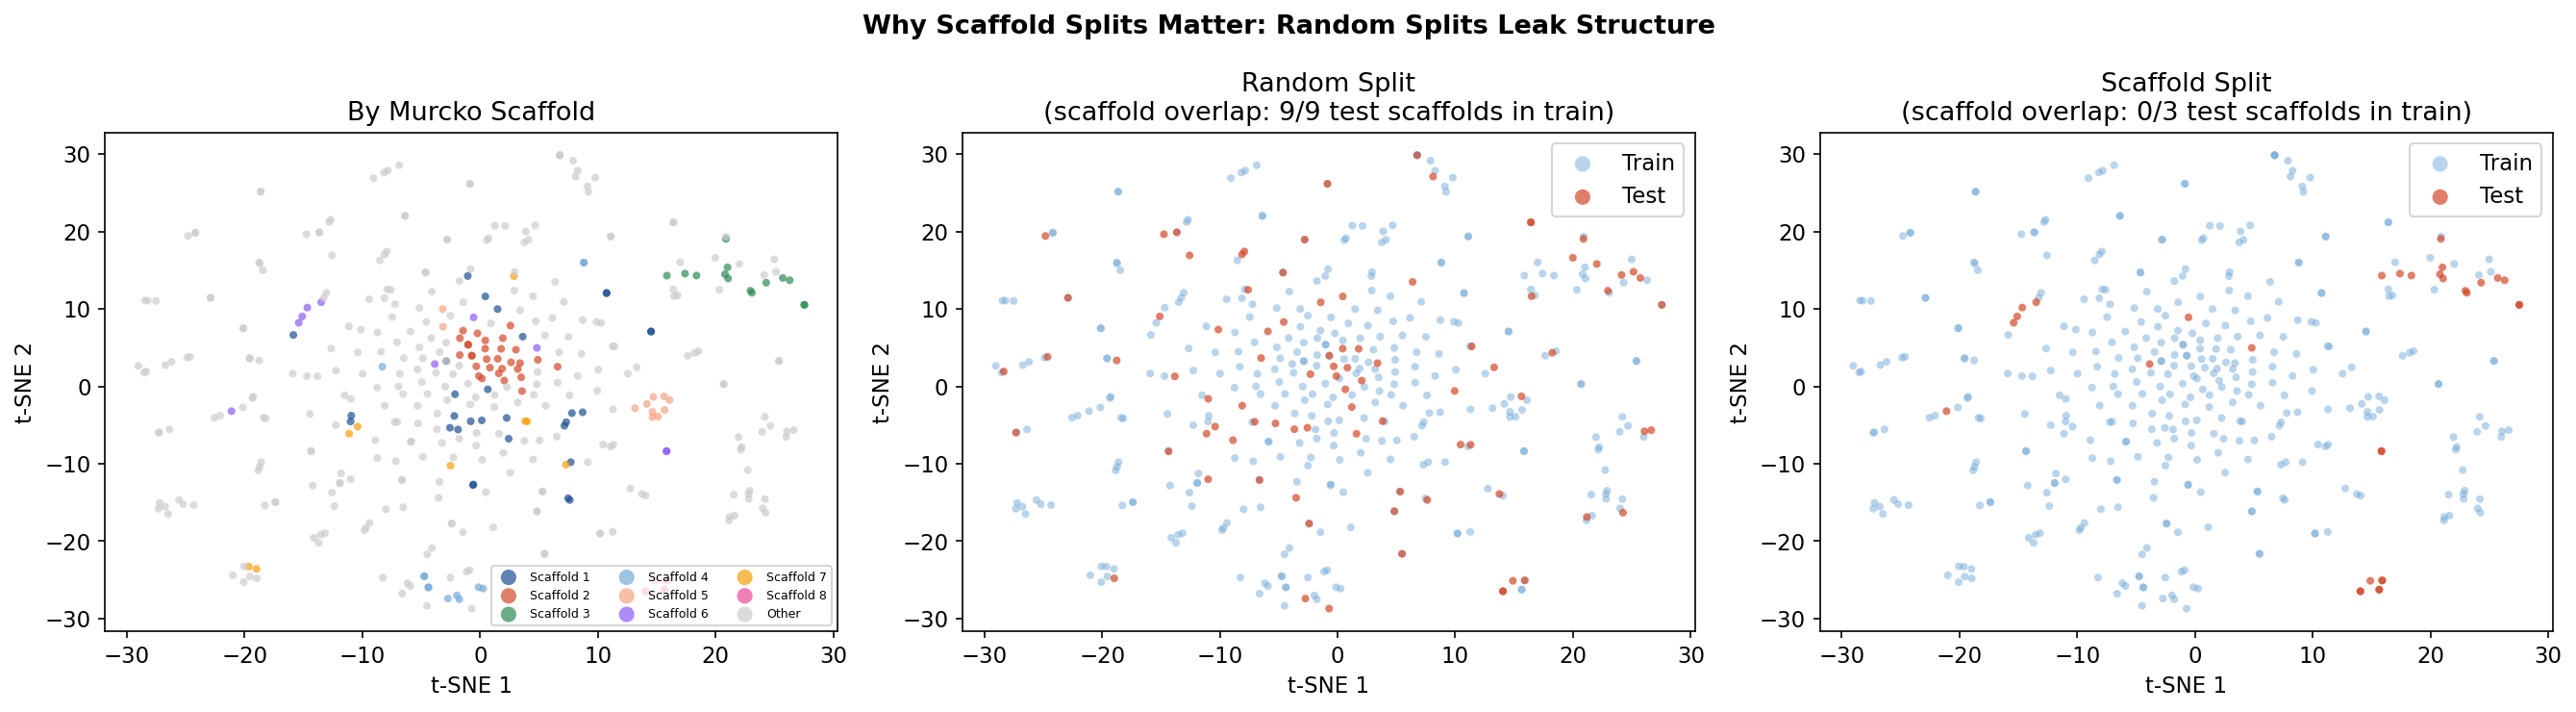
\includegraphics[width=0.92\textwidth,height=0.72\textheight,keepaspectratio]{fig5_scaffold_split.png}
\end{center}
\vspace{-0.5em}
{\scriptsize [Notebook Fig.~5] Left: molecules colored by Murcko scaffold. Middle: random split---scaffolds leak across train/test. Right: scaffold split---test scaffolds are entirely unseen during training.}
\end{frame}

% ============================================================
\begin{frame}{Molecular Docking}
\textbf{This is where proteins and small molecules meet:} given a protein structure and a candidate drug, predict how and how well they bind.

\vspace{0.1em}
\begin{center}
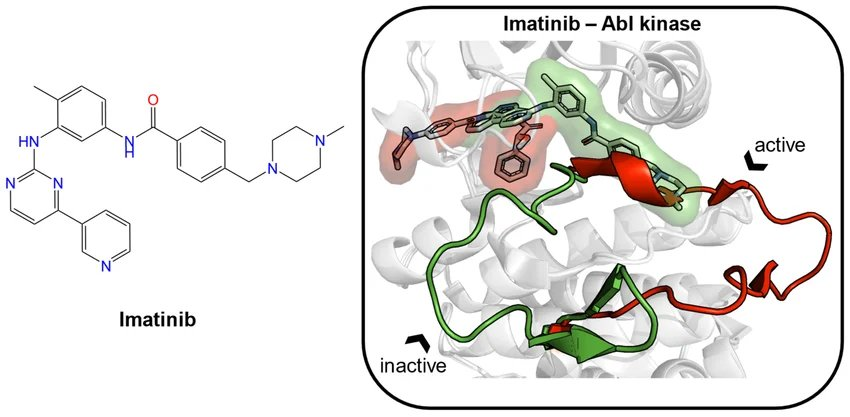
\includegraphics[width=0.85\textwidth,height=0.38\textheight,keepaspectratio]{imatinib_docking.png}
\end{center}
\vspace{-0.3em}
{\scriptsize Imatinib (Gleevec) bound to Abl kinase (PDB: 1IEP). Left: 2D structure. Right: drug in the binding pocket---shape complementarity in action.}

\pause
\vspace{0.1em}
{\footnotesize \textbf{Virtual screening:} Dock millions of candidates, test top hits. Scoring: force-field-based, empirical, or knowledge-based. Useful for filtering and hypothesis generation, but raw docking scores $\neq$ true binding affinity.}
\end{frame}

% ============================================================
\section{Integration}
% ============================================================

\begin{frame}{The Drug Discovery Pipeline}
\begin{center}
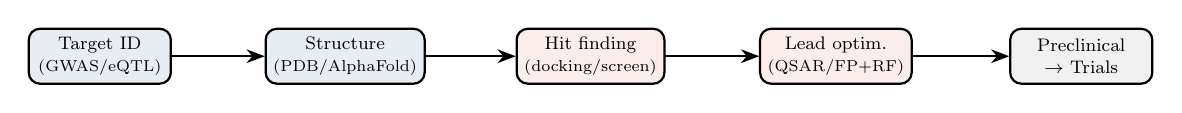
\begin{tikzpicture}[
    box/.style={draw,thick,rounded corners,minimum width=2.2cm,minimum height=0.85cm,align=center,font=\footnotesize},
    >=Stealth,scale=0.82,transform shape
]
\node[box,fill=columbia!10] (target) at (0,0) {Target ID\\{\scriptsize (GWAS/eQTL)}};
\node[box,fill=columbia!10] (struct) at (3.8,0) {Structure\\{\scriptsize (PDB/AlphaFold)}};
\node[box,fill=columbiaaccent!10] (hit) at (7.6,0) {Hit finding\\{\scriptsize (docking/screen)}};
\node[box,fill=columbiaaccent!10] (lead) at (11.4,0) {Lead optim.\\{\scriptsize (QSAR/FP+RF)}};
\node[box,fill=columbiagray!10] (trial) at (15.2,0) {Preclinical\\$\to$ Trials};
\draw[->,thick] (target) -- (struct);
\draw[->,thick] (struct) -- (hit);
\draw[->,thick] (hit) -- (lead);
\draw[->,thick] (lead) -- (trial);
\end{tikzpicture}
\end{center}

\vspace{0.3em}
Where classical methods fit at each step:
\begin{itemize}[<+->]
    \item \textbf{Target:} GWAS $\to$ eQTL $\to$ which protein to target
    \item \textbf{Structure:} Homology modeling, experimental methods
    \item \textbf{Hit finding:} Docking, virtual screening
    \item \textbf{Lead optimization:} QSAR, fingerprint similarity
\end{itemize}
\end{frame}

% ============================================================
\begin{frame}{Classical Methods: Baselines to Beat or Build Upon}

\vspace{0.2em}
\begin{center}
{\footnotesize
\renewcommand{\arraystretch}{1.1}
\begin{tabular}{lll}
\toprule
\textbf{Task} & \textbf{Classical method} & \textbf{Strength} \\
\midrule
Variant effect & SIFT, PolyPhen, REVEL, CADD & Widely used, strong baselines \\
Structure prediction & Homology modeling & Works if template exists \\
Molecular similarity & Morgan FP + Tanimoto & Fast, no training needed \\
Property prediction & FP + RF & Often competitive on small data \\
Binding prediction & Docking & General-purpose baseline \\
\bottomrule
\end{tabular}
}
\end{center}

\pause
\vspace{0.2em}
{\small Note: the MSA is not only a classical method---it remains a \emph{critical input} to the best DL models. AlphaFold~2's Evoformer explicitly consumes MSA columns. Classical and DL are not always in competition; often the best systems integrate both.}
\end{frame}

% ============================================================
\begin{frame}{Key Takeaways}
\begin{itemize}[<+->]
    \item \textbf{MSA is the foundation} of classical protein analysis --- conservation, coevolution, variant prediction, homology modeling all flow from it
    \item \textbf{Coevolution} encodes implicit 3D information --- AlphaFold~2 uses this explicitly via MSAs; protein LMs learn related constraints from large sequence corpora
    \item \textbf{SMILES and fingerprints} are molecular baselines; FP+RF is embarrassingly strong
    \item \textbf{Activity cliffs} show that structural similarity $\neq$ functional similarity
    \item \textbf{Scaffold split} is the molecular patient-level split --- evaluation $>$ model choice
    \item \textbf{Classical $+$ DL:} the best systems integrate classical tools (MSAs, fingerprints) with learned representations
\end{itemize}
\end{frame}

% ============================================================
\begin{frame}{Acronyms and Tools Introduced Today}
\begin{center}
{\footnotesize
\renewcommand{\arraystretch}{1.05}
\begin{tabular}{ll}
\toprule
\textbf{Acronym} & \textbf{Full Name} \\
\midrule
BLAST & Basic Local Alignment Search Tool \\
PSI-BLAST & Position-Specific Iterated BLAST \\
HMM & Hidden Markov Model \\
PSSM & Position-Specific Scoring Matrix \\
DCA & Direct Coupling Analysis \\
SIFT & Sorting Intolerant From Tolerant \\
PolyPhen & Polymorphism Phenotyping \\
CADD & Combined Annotation Dependent Depletion \\
REVEL & Rare Exome Variant Ensemble Learner \\
SMILES & Simplified Molecular-Input Line-Entry System \\
ECFP / Morgan & Extended-Connectivity Fingerprint \\
QSAR & Quantitative Structure--Activity Relationship \\
\bottomrule
\end{tabular}
}
\end{center}
\end{frame}

% ============================================================
\begin{frame}[standout]
    Questions?
\end{frame}

\end{document}
